\documentclass[11pt,a4j]{jarticle}

\newcommand{\setcounters}[1] {
  \setcounter{equation}{#1}
  \setcounter{figure}{#1}
  \setcounter{table}{#1}
}

\newcommand{\unit}[1] {
  \hspace{1mm}\mathrm{[#1]}
}

\newcommand{\degc} {
  \hspace{1mm}\mathrm{[}{}^\circ\mathrm{C]}
}

\newcommand{\refig}[1]{図\ref{fig::#1}}
\newcommand{\refeq}[1]{式(\ref{eq::#1})}
\newcommand{\reftab}[1]{表\ref{tab::#1}}

\newcommand{\fig}[5] {
  \begin{figure}[#1]
    \begin{center}
      \includegraphics[width=#2\hsize]{#3}
    \end{center}
    \caption{#4}
    \label{fig::#5}
  \end{figure}
}

\makeatletter
\def\eq{\@ifstar\@eq\@@eq}
\def\@eq#1{\begin{equation*}#1\end{equation*}}
\def\@@eq#1#2{\begin{equation}#2\label{eq::#1}\end{equation}}
\makeatother

\newcommand{\diff}[2] {
  \frac{\mathrm{d}#1}{\mathrm{d}#2}
}

\newcommand{\pdiff}[2] {
  \frac{\partial #1}{\partial #2}
}


\newcommand{\ddt}[2][1] {
  \ifnum #1 < 2
    \frac{\mathrm{d}#2}{\mathrm{d}t}
  \else
    \frac{\mathrm{d}^#1#2}{\mathrm{d}t^#1}
  \fi
}

\newcommand{\e}[1] {
  \mathrm{e}^{#1}
}

\newcommand{\lparen}{(}
\catcode `( = \active
\newcommand{(}{\ifmmode\left\lparen\else\lparen\fi}

\newcommand{\rparen}{)}
\catcode `) = \active
\newcommand{)}{\ifmmode\right\rparen\else\rparen\fi}

\newcommand{\bmat}[1] {
  \begin{bmatrix} #1 \end{bmatrix}
}

% -- Package ---------------------------------------------------
\usepackage[dvipdfmx]{graphicx}
\usepackage{amsmath, amssymb}
\usepackage{bm}
\usepackage{fancyhdr}
\usepackage{here}
\usepackage{listings}
\usepackage{multirow}


% -- Margin Config ---------------------------------------------
\setlength{\textheight}{\paperheight}
\setlength{\topmargin}{4.6truemm} % 30mm(=1.0in+4.6mm)
\addtolength{\topmargin}{-\headheight}
\addtolength{\topmargin}{-\headsep}
\addtolength{\textheight}{-60truemm}

\setlength{\textwidth}{\paperwidth}
\setlength{\oddsidemargin}{-0.4truemm} % 25mm(=1.0in-0.4mm)
\setlength{\evensidemargin}{-0.4truemm}
\addtolength{\textwidth}{-50truemm}


% -- Renewcommand ----------------------------------------------
\renewcommand{\theequation}{\arabic{section}.\arabic{equation}}
\renewcommand{\thefigure}{\arabic{figure}}
\renewcommand{\thetable}{\thesection.\arabic{table}}
\renewcommand{\lstlistingname}{ソースコード}
\renewcommand{\headrulewidth}{0mm} % fancy
\renewcommand{\labelenumi}{(\arabic{enumi})}


% -- Config for fancy package ----------------------------------
\pagestyle{fancy}
\rhead{\thepage}
\lhead{}
\cfoot{}


% -- Config for package listings -------------------------------
\lstset{
  basicstyle={\ttfamily \small},
  breaklines=true,
  frame=trBL,
  numbers=left,
  numberstyle={\ttfamily \small},
}




\begin{document}
\begin{titlepage}

  \vspace*{25mm}

  \begin{center}
    {\huge 知能制御PBL\\}
    \vspace{10mm}
    {\Huge 第2回RCR中間報告\\}
    \vspace{20mm}
    {\Large 2018年6月6日}

    \vspace{15mm}

    {\LARGE 西田研究室\\}

    \vspace{15mm}

    {\Large
   13104042 烏谷崇大    \\
   14104055 佐々木秀将\\
   15104021 長田駿二郎\\
   15104026 川崎雄太朗\\
   15104050 坂元勇太    \\
   15104081 徳野将士    \\
   15104113 前田修一    \\
   15104117 右田明花    \\
   15104134 山福佳        \\
   17104311 横田篤紀    \\
}

  \end{center}

\end{titlepage}


\newpage
	\tableofcontents

\newpage
\section{目的}
	学部3年までに学習した制御理論や電気回路・情報工学の知識を使って,競技場内を自律的に走行するロボットの製作を行う.
	研究室で一丸となってプロジェクトを進行し,共同で課題を達成することの難しさや楽しさを学び,エンジニアとして仕事を進めるための素養を身に付ける.

\section{ROS}
\subsection{ROSとは}
ROS(Robot Operating System)とはOpen Source Robotics Foundationによって管理されているソフトウェア開発者のロボット・アプリケーション作成を支援するフレームワークである.
具体的には,ハードウェア抽象化,デバイスドライバ,ライブラリ,視覚化ツール,メッセージ通信,パッケージ管理などが提供されている.
つまりROSは汎用コンピュータ向けのOSではなく,汎用コンピュータ向けOS上で動作するメタOSとして捉えることができる\cite{kurazume}.

\refig{ros_topic}に示すようにROSではプロセス(実行プログラム)はノードという単位で扱い,ノード間の通信はトピックと呼ばれる``Publisher/Subscriber''モデルで実現される\cite{ogura}.

これにより,プログラミング言語や通信相手さえ意識することなく簡単にプロセス間通信を実現できる.
これは各ノード間のインタフェース,即ちトピックの名前と型さえ決定すればノードごとに独立して開発を行うことができるという利点でもある.\\

以上の利点を鑑み,本研究室ではROSがインストール可能なマイコンボードであるRaspberryPi3 Model B上にROSをインストールして開発を進めていくこととした.

\begin{figure}[htb]
  \centering
    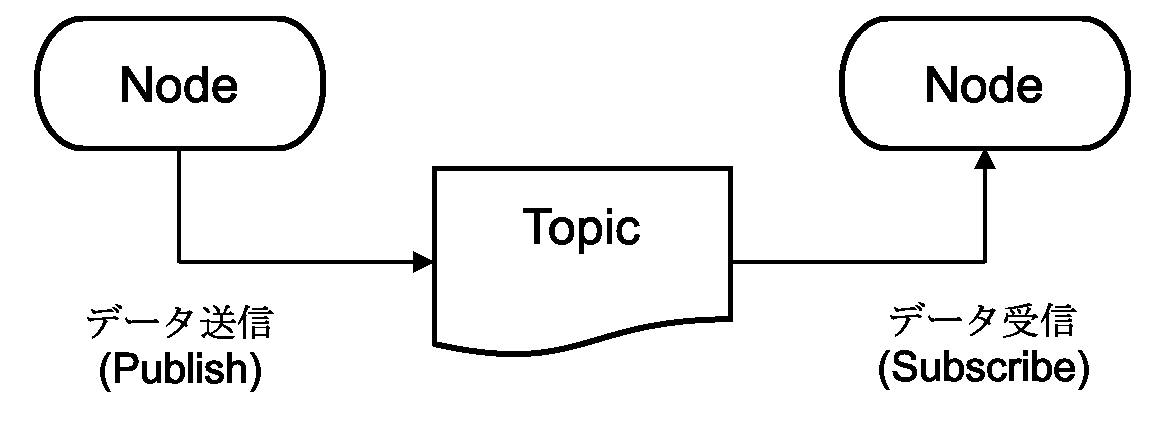
\includegraphics[width=0.5\hsize]{picture/eps/ros_topic.eps}
    \caption{ROSノードとトピックの概念}
    \label{fig::ros_topic}
\end{figure}



\begin{figure}[htb]
  \centering
    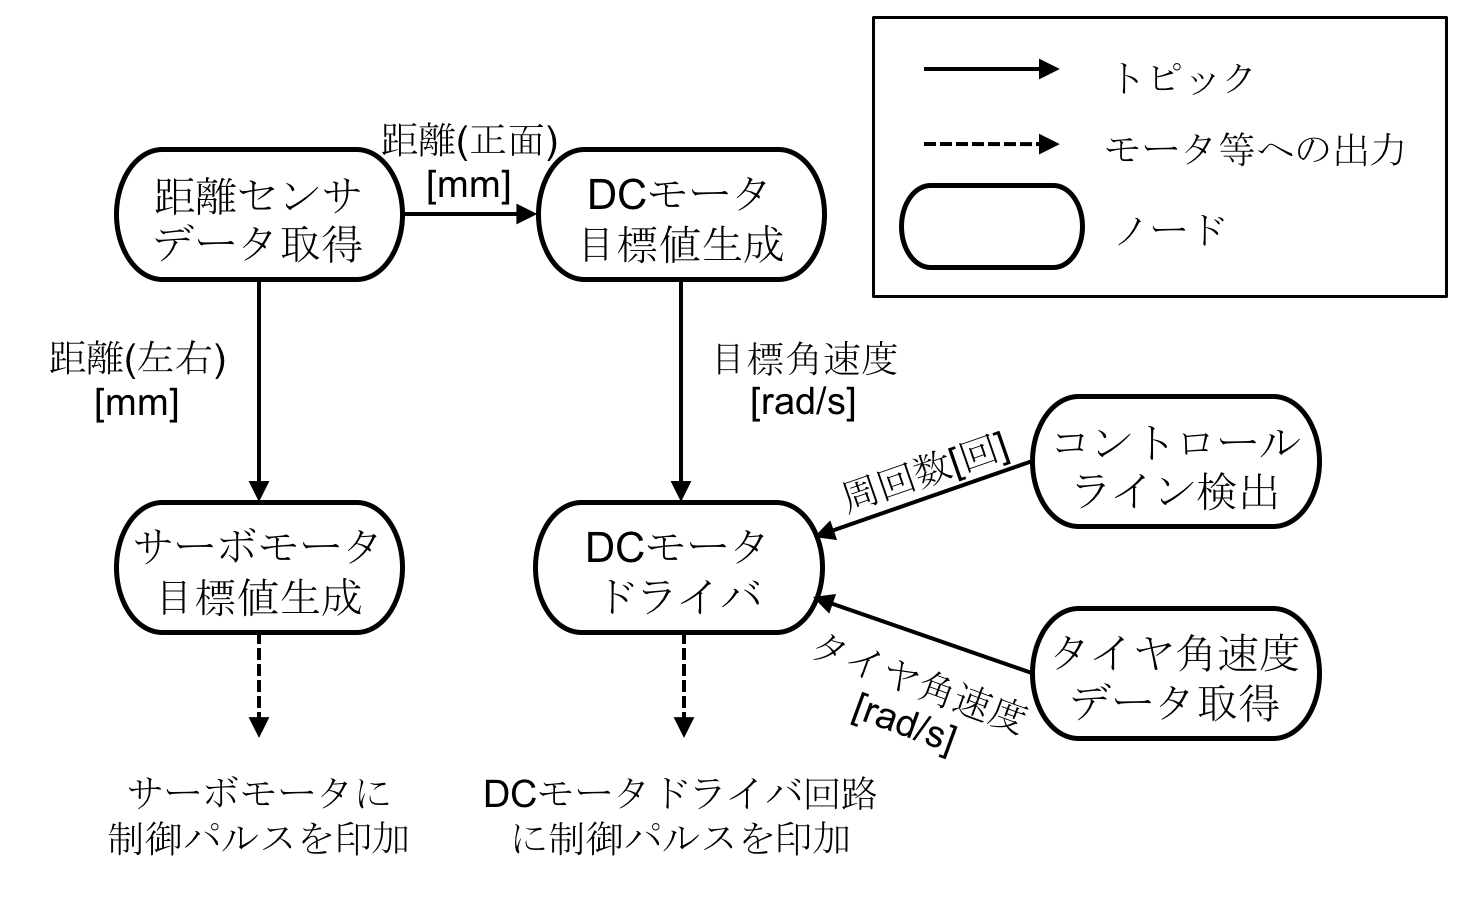
\includegraphics[width=0.8\hsize]{picture/eps/ros_nodes.eps}
    \caption{ROSノードとトピックの構成}
    \label{fig::ros_nodes}
\end{figure}

\newpage
\subsection{ROSノードとトピックの構成}
\refig{ros_nodes}に開発するROSノードとトピックの構成を示す.各ノードの役割は次の通りである.
\begin{description}

    \item[距離センサデータ取得] \mbox{} \\
      機体前方及び両側面に設置した距離センサからシリアルバス規格の一つである$\mathrm{I^2C}$を介して距離データを$\mathrm{[mm]}$単位で取得し外れ値処理や正規化を施した後にPublishする.
    \item[コントロールライン検出] \mbox{} \\
      機体後方下部に設置したフォトリフレクタによってコントロールラインを通過した回数をカウントしPublishする.

    \item[タイヤ角速度データ取得] \mbox{} \\
      回転方向は考慮しないため,ロータリーエンコーダのA相のパルスのみをカウントし,ロータリーエンコーダの一周あたりの出力パルス数$(500パルス)$,サンプリング周期$(0.01\unit{s})$,ロータリーエンコーダの軸に取り付けたピニオンギアとドライブシャフトに取り付けたギア間のギア比$(2.74)$を考慮して$k$時点のタイヤの角速度$\omega(k)$を$\unit{rad/s}$単位で算出する.また,ノイズ対策として算出した角速度を\refeq{lpf}で表されるデジタルフィルタ(LPFに相当)に通した結果をPublishするようにしている.ただし,$\alpha$は$0〜1$の範囲で定める定数である.\\
      \begin{equation}
      	\omega(k)=\alpha\omega(k)+(1-\alpha)\omega(k-1)\label{eq::lpf}
      \end{equation}

    \item[DCモータ目標値生成] \mbox{} \\
      機体前方方向の距離データをSubscribeし,それをもとにDCモータに与える目標値を生成しPublishする.

    \item[DCモータドライバ] \mbox{} \\
      DCモータに与える目標値とタイヤの角速度データをSubscribeし,PI制御則に基づきDCモータを駆動する.

    \item[サーボモータ目標値生成] \mbox{} \\
      機体前方の距離データをSubscribeし,それをもとにサーボモータに与える目標値を生成しその後直接サーボモータを駆動する.サーボモータドライバノードが存在しないのはサーボモータの軸にロータリーエンコーダがついておらず角度フィードバックが出来ないためである.

  \end{description}

\begin{thebibliography}{9}
 \bibitem{kurazume}
    表允晳,倉爪亮,渡邊裕太, ``詳説 ROSロボットプログラミング-導入からSLAM・Gazebo・MoveItまで-'', \\
    Kurazume Laboratory, pp.15-18, (2015).

  \bibitem{ogura}
    小倉崇, ``ROSではじめるロボットプログラミング'', 工学社, pp.8-10, (2015).

\end{thebibliography}


\end{document}
